\chapter{Literature}\label{ch:literature}
		This Chapter presents \gls{cawiml} as an alternative authoring language to specify questionnaires only using standard \gls{xml} schema languages. Particularly, it uses a state-transition paradigm for question's sequence and is intended to facilitate the questionnaire routing logic more adequately than the popular hierarchical model. \gls{rpn}, is the expression formalism utilised for describing routing and personalisation constructs indistinctly.

	The rest of this Chapter is structured as follows: Section \ref{sec:cawiLanguage:stateTransition} introduces the state-transition routing structure. Section \ref{sec:cawiLanguage:rpn} explains the postfix notation mode as the formalism for questionnaire expressions, followed by Section \ref{sec:cawiLanguage:xmlLanguage} that explains our \gls{xml} authoring solution. Finally, \gls{xml} details for content, routing and personalisation constructs expressed in \gls{cawiml} are presented in Section \ref{sec:cawiLanguage:cawiml}.
	 
\section{The XML Languages}\label{sec:literature:xmlLanguages}
		The most relevant \gls{xml} languages addressed to cover questionnaire constructs are \gls{triples}, \gls{sss}, \gls{qdl} and \gls{ddi}. The following sections provide a brief description of each authoring solution before conducting a comparative analysis.

	\subsection{Survey Interchange Standard (Triple-S)}
			%Triple-S is aimed to describe the key elements of surveys \cite{book:triplesxml} in order to make easier the transfer of data and meta data between survey or analysis software packages. Wright describes an use case tool which accepts data in triple-S format to take business decisions \cite{proc:wright07}.

	%This language was first published in 1994 and since then three major versions have been released. The latest one (2.0) defines two files: the \emph{definition File} which contains general information and survey variables (i.e. the meta data) and the \emph{Data File} storing data for a meta data instance. This version supports \gls{csv} format for exporting the survey data as well as the ability to specify hierarchies. The hierarchy feature results useful for questionnaires where exist a relationship parent-children (e.g. a household questionnaire contains questions at the household level and a set of questions to be repeated for each member of the household). This relationship is defined through a specification control file.

	\gls{triples} is aimed to represent the content aspects of surveys \cite{book:triplesxml} in order to make it easier to transfer data and meta data among \gls{cai} systems or any analysis software package. This language is considered the standard for representing social surveys and at least fifty registered implementers may be found on its website \cite{web:triples}. Although its focus has been to provide a comprehensive coverage of survey functionality, we have found one case study where \gls{triples} has been adapted to describe a business decision making tool \cite{proc:wright07}.
	\subsection{Questionnaire Definition Language (QDL)}
			%\gls{qdl} is an \gls{xml} language developed as part of the \gls{tadeq} project. \gls{tadeq}'s aim is building a software tool for translating questionnaire specifications from different \gls{cai} systems in a human-readable format \cite{proc:bethlehem00}. This tool is able to generate two types of documentation: \emph{textual}, providing detailed information on all questionnaire constructs and \emph{graphical}, assisting in the understanding of the routing structure. The tool attempts to be helpful for different target people: \emph{questionnaire developers} who want to document their work, \emph{survey managers} who have to give formal approval to execute the survey and \emph{interviewers} who want the documentation to help them when they are collecting responses.

	%\gls{tadeq} accepts \gls{xml} instances according to \gls{qdl} which means every \gls{cai} survey system has to create its own converter from its authoring questionnaire language to \gls{qdl} (e.g. Blaise system has its own converter). \gls{qdl} is focused on design and collection stages of surveys and is able to describe filter and skip constructs indistinctly.

	\gls{qdl} is a language built for \gls{tadeq} project whose aim is at building a software tool that represents questionnaire specifications in a human-readable format \cite{proc:bethlehem00}. This tool can operate in either textual or graphical mode. It is suited to designers who want detailed information of the constructs and interviewers who need documentation to help them when they are conducting interviews. Although this project has some implementers like Blaise that has its own converter, this project has been abandoned and there is no longer support for this language.





	\subsection{Data Documentation Initiative (DDI)}
			\gls{ddi} emerged in 1995 as an international project to create standardised meta data to document social science datasets \cite{art:rasmussen07}. It emerged to solve the problems of documenting datasets and introduces \gls{xml} as the exchangeable data format to be both, machine-readable and human-understandable. It has an important value for analysis and archiving since permits describing data at two levels: \emph{variable} level, which consist of describing the different variables involved on the research; and \emph{study level}, since it allow describing the population that links to the stored information. 

	In its third version was introduced the description of social surveys. Since then, the \gls{abs} has been experimenting with this exchangeable format for their design tool for questionnaires. Similarly, \gls{insee}, that uses Blaise \gls{cai} system for collecting data has shown interest on using \gls{ddi} as a standard to communicate different disciplines in the data collection field. For that purpose, a \gls{pof} was created by de Bolster to convert from Blaise language specifications to \gls{ddi} 3.1. From that experiment, it was concluded that neither \gls{ddi} instances are human readable nor compatibility between different versions is considered. For instance, when valid \gls{ddi} instances for questionnaires were verified against the schemas of the newer version at least 365 errors occurred \cite{proc:bolster13}.
	\subsection{Simple Survey System (SSS)}
			%-The response data is stored in XML files
	%-The survey engine runs C++.
	%-Rules are defined in \gls{xsd}.
	%-Number and type of arguments cannot be validated when the questionnaire specification file is read. Argument validation must wait until the function is actually invoked.
	%-Expressions are evaluated recursively from inside out.
	%-Functional approach leds to expressive structurefor representing calculations and expressions

	%\gls{sss}, known as a \gls{capi} system solution developed for \gls{rti} which has its own \gls{xml} specification language to address the questionnaire constructs \cite{art:bethke08}.
	%This language has a different approach to define its logical and arithmetical expressions based on a functional programming style which makes the authoring language more robust and less prone errors.
	\gls{sss} is a \gls{capi} system solution developed for \gls{rti} which has its own \gls{xml} language to address content, routing and personalisation features of surveys \cite{art:bethke08}. This language unlike \gls{triples}, \gls{qdl} or \gls{ddi} has a robust schema to represent the logical and arithmetical expressions based on functional programming style. 


\section{Comparative Analysis of XML Languages}\label{sec:literature:comparativeAnalysis}
		In this section we detail a comparative analysis of the \gls{xml} authoring languages used to define questionnaire specifications. For that purpose, we explore the coverage of routing and personalisation constructs in Section \ref{sec:literature:routing} and \ref{sec:literature:personalisation} respectively. The relevant flow paradigms used to capture the routing sequence for questionnaires is explained in Section \ref{sec:literature:flowParadigm}. The constraining level coverage of the schema languages used to define these \gls{xml} languages is addressed in Section \ref{sec:literature:schemaLanguages}. Section \ref{sec:literature:expressionNotation} studies the three notation to describe logical and arithmetical expressions through an example from a real questionnaire and finally the survey life-cycle stages in which every \gls{xml} language is focused on is detailed in Section \ref{sec:literature:surveyStages}. Table \ref{tab:literature:comparison} summarises the above mentioned aspects that will be treated on the next sections.

	\begin{sidewaystable}
	\begin{center}
	\begin{tabular}{|c|c|c|c|c|c|}
	\hline 
	\textbf{\textcolor{blue}{\emph{Category}}} & \textbf{\textcolor{blue}{\emph{Feature}}} & \textbf{\textcolor{blue}{\emph{Triple-S}}} & \textbf{\textcolor{blue}{\emph{SSS}}} & \textbf{\textcolor{blue}{\emph{QDL}}} & \textbf{\textcolor{blue}{\emph{DDI}}}\tabularnewline
	\hline 
	\hline 
	\multirow{5}{*}{\textbf{\textcolor{blue}{\emph{Routing}}}} & \textbf{Skip} & No & No & Yes & No\tabularnewline
	\cline{2-6} 
	 & \textbf{Filter} & Partial & Yes & Yes & Yes\tabularnewline
	\cline{2-6} 
	 & \textbf{Loop} & No & Yes & Partial & Yes\tabularnewline
	\cline{2-6} 
	 & \textbf{Check} & No & No & Yes & No\tabularnewline
	\cline{2-6} 
	 & \textbf{Computation} & No & Yes & Yes & Yes\tabularnewline
	\hline 
	\multirow{4}{*}{\textbf{\textcolor{blue}{Personalisation}}} & \textbf{Piping - text-fill} & No & Yes & No & Yes\tabularnewline
	\cline{2-6} 
	 & \textbf{Piping - carry-forward} & No & No & No & No\tabularnewline
	\cline{2-6} 
	 & \textbf{Randomising} & No & No & No & Partial\tabularnewline
	\cline{2-6} 
	 & \textbf{Rotating} & No & No & No & Partial\tabularnewline
	\hline 
	\multirow{4}{*}{\textbf{\textcolor{blue}{\emph{Other}}}} & \textbf{Flow Paradigm} & N/A & Hierarchical & Hierarchical & Hierarchical\tabularnewline
	\cline{2-6} 
	 & \textbf{XML Schema Language} & DTD & XSD 1.0 & DTD & XSD 1.0\tabularnewline
	\cline{2-6} 
	 & \textbf{Expressions Notation} & N/A & PreFix & Infix & Infix\tabularnewline
	\cline{2-6} 
	 & \textbf{Survey Stage} & Analysis/Reporting & Design/Collection & Design & Analysis/Reporting\tabularnewline
	\hline 
	\end{tabular}
	\caption{Comparison of XML languages for electronic questionnaires}
	\label{tab:literature:comparison}
	\end{center}
	\end{sidewaystable}
	\subsection{Routing Constructs}\label{sec:literature:routing}
			The filter construct is well represented by \gls{sss}, \gls{qdl} and \gls{ddi} whereas it is partially described by \gls{triples} since this language is only able to represent simple logic involving only one variable. 

	In contrast, the skip logic is only defined by \gls{qdl} which considers the fact that for questionnaire designers it is difficult to express conditional statements \cite{proc:katz97}. However, as far as we know, the tool that implements this language does not offer support since it is difficult to implement conditions without having restrictions over the type of jumps allowed \cite{art:bethlehem04}. The other languages do not cover this construct either because the skips can be reversed and use filters instead \cite{art:bethke08} or since surveys designed without unstructured patterns are easy to modify, share and understand \cite{web:spencer12}. %NOT CLEAR SKIP REVERSED AND USE FILTERS INSTEAD

	The loop construct is well represented in \gls{sss} and \gls{ddi}. Despite the fact that \gls{ddi} offers three types of loops (RepeatUntil, RepeatWhile and range loop) \cite{man:thomas09}, we consider that \gls{sss} is more flexible than \gls{ddi} to define expressions since it embodies a simple functional programming style through the use of \gls{xml} tags. In spite of \gls{qdl}, it only offers support for range loop but does not consider iterations over lists (see the instruction after Q5 in Figure \ref{fig:background:survey}). Regarding \gls{triples}, it does not directly define any mechanism to iterate, although offers an interesting feature to relate data collected from hierarchical surveys (e.g. survey responses for a household survey followed by responses of the property members defined in another survey) \cite{proc:wright07}.

	The check construct is only featured in QDL and this is likely to be motivated by the need to describe multi-item constraints to check consistencies among answers to related questions \cite{proc:katz97} or alternatively because this XML language is strongly related to Blaise system \cite{proc:bethlehem00}. Regarding the computation feature, other than Triple-S, all others languages support its representation.

	\subsection{Personalisation Constructs}\label{sec:literature:personalisation}
			Although \gls{sss} and \gls{ddi} offer mechanisms to describe \emph{text-fill} aspects, the other piping feature, i.e. the \emph{carry-forward} has not been considered. This construct, which permits describing operations to retrieve selected on unselected responses from previous questions as part of the responses for other questions (see Q3 from Figure \ref{fig:background:survey}), may help to better adapt surveys for each respondent. Accordingly, we consider that a specification language cannot leave out this construct. For instance, the popular SurveyMonkey \gls{cawi} system, we have observed that it implements this personalisation feature as part of its interface functionalities.

	Regarding the randomising and rotating features, these constructs are only partially covered by \gls{ddi} permitting to change the order for content constructs such as single and/or multiple question responses. However, more sophisticated patterns like selecting a specific number of responses after randomising/rotating or reordering only a subset of responses is not taken into account. For instance, the instruction above Q6a from Figure \ref{fig:background:survey} not only specifies to randomise the elements selected but also requires to iterate a maximum of four times.

	\subsection{Routing Flow Paradigms}\label{sec:literature:flowParadigm}
			The questionnaire's flow captures the sequence for the question constructs defined in a questionnaire. The designers or social researchers commonly use skip patterns that can be interchanged with filters to express the logical order of elements in a questionnaire. We have explored the directed graphs, Petri Nets and the hierarchical paradigms in order to %find out whether these approaches describe questionnaires in a structured manner but permitting designers to express logics through skip patterns.
	establish the suitability for representing sequence logic.

	The \emph{directed graph}, was explored in the past by Fagan et al. in order to analyse the use of skip constructs on surveys. These graphs based on \emph{nodes} and \emph{arcs} are able to represent question and response choices respectively. %Moreover, the source and sink properties of the graph correspond to the first and last question of a questionnaire. 
	When additional information such as the conditions that determine the ordering of questions are added to these graphs, they become flowcharts which result in tools to document and understand questionnaire's flow \cite{art:jabine85}. The directed graphs, permit validating the correctness of data gathered from surveys by detecting whether or not a question response is missed or is not applicable. These verifications are conducted applying different graph properties \cite{tech:fagan88}. Although the properties from graphs can be used to model the flow of questionnaires, as far as we know, this paradigm has not been used to formally define questionnaire specifications in \gls{xml}.

	In more recent work, Petri Nets have been applied to visualise and analyse complex questionnaires \cite{proc:rolke10}. Figure \ref{fig:literature:pretiNet} illustrates the Petri Net representation on part of the questionnaire from Figure \ref{fig:background:survey} in relation to question Q1 and the skip construct that permit navigating either to Q2 or END. %A more recent study case carried out by Rolke is concentrated on the visualisation and analysis of a complex questionnaire using Preti Nets. Figure \ref{fig:literature:pretiNet} contains a small portion of this net that represents part of the paper questionnaire from Figure \ref{fig:background:survey}. Specifically, it is depicted the question Q1 and the skip construct that permit navigating either to Q2 or END. 
	Here a \emph{place} (e.g. Q1, Q2 and END) captures the static information from a question whereas a transition (e.g. 01, 02, 03, 04, 05) represents a response choice. Additionally exist \emph{arcs} to connect places to transitions (e.g. arrow connecting Q1 to 01) and vice versa (e.g. 01, 02 and 03 to END). A Petri Net permits validating the \emph{reachability} of places, i.e. checking whether or not a set of responses given for questions correspond to a valid state of the net. However, this modelling approach is only limited to finite domain, i.e. it is only applicable for single and multiple questions, but becomes hard to manage open questions since an arc connecting places to/from transitions has to be specified for any possible value expected.

	\begin{figure}[h]
	\centering
	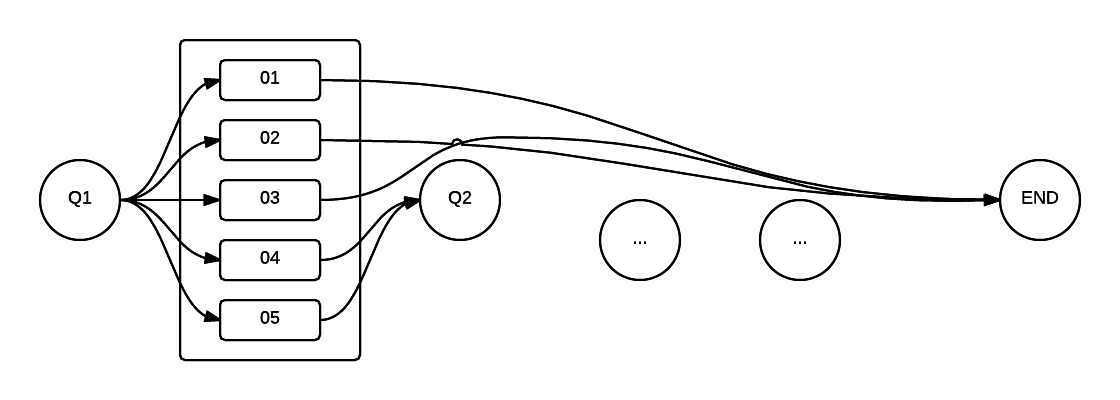
\includegraphics[max size={\textwidth}{\textheight}]{literature/img/pretiNet.png}
	\caption{Petri Net instance}
	\label{fig:literature:pretiNet}
	\end{figure}

	\gls{sss}, \gls{ddi} and \gls{qdl} adopt a hierarchical modelling approach where the use of skip pattern is avoided in favour of structured constructs (if-then-else, loops and sequences) as advocated by Dijkstra \cite{art:dijkstra68}. As such, the routing structure of surveys can be seen as trees permitting not only the identification of the path followed but also determining all the circumstances under which a question may be triggered \cite{web:spencer12}. Algorithm \ref{alg:hierarchical} describes in pseudo-code the routing of the questionnaire from Figure \ref{fig:background:survey} according to the hierarchical modelling. Note how the nesting of constructs is used to avoid skips. However, this nesting is not naturally well suited to reusability.%WEIRD does not naturally well suited ...

	\begin{algorithm}
	INF1\;
	Q1\;
	\If{NOT(Q1 IS\_SEL '01' OR Q1 IS\_SEL '02' OR Q1 IS\_SEL '03')}{
		Q2\;
		\If{NOT(Q2 IS\_SEL '99')}{
			Q3\;
			\If{NOT(Q3 IS\_SEL '99')}{
				Q4\;
				\If{Q2 IS\_SEL '06'}{
					Q5\;
					\For{each Q2 SEL}{
						Q6a\;
					}
					\If{HAD\_CAR \textgreater 1}{
						INF2\;
					}
				}
			}
		}
	}
	END\;
	\caption{Hierarchical modelling example}
	\label{alg:hierarchical}
	\end{algorithm}

	The benefits of eliminating skip patterns are universally acknowledged by high-level programme languages architects, however designers or social researchers still specify questionnaires through documents using skips to navigate from one question to another \cite{proc:katz97}, not only because they do not have programming skills but also because the final client interested in the survey, demands plain English instructions. As the hierarchical approach replaces the use of skip constructs, there is an evident \emph{gap} between what the social researchers design versus the \emph{code} that a \gls{cawi} system uses to execute a survey. Costigan states that having two sources of specification, i.e. the code and the document requires duplication of effort and it is prone to error \cite{proc:costigan03}. To unify these two sources, Spencer proposes that researchers should be trained to use structured patterns \cite{web:spencer12}, i.e. avoid the use of skip constructs. However, in practice, motivating social researchers to adopt this practice remains a problem \cite{proc:costigan03}. %few social researchers would be interesting in eliminating skip patterns from questionnaire specifications \cite{proc:costigan03}.

	The ability to introduce changes to questionnaires is another factor to consider since clients often demand the modification of survey logics when the data collection is already taking place. This involves having a modelling approach that addresses the \emph{adaptability} appropriately. It is evident from the above hierarchical representation that strong coupling between the inner and outer filters increases with increasing skip constructs. %It is evident by examining the above example introduced, that exist coupling between the inner and outer filters which increases when newer skip constructs are added. 
	As dependencies among constructs are like to impact negatively to changes to questionnaire's flow, there is a need to explore a less intrusive model.
	

	\subsection{Schema Languages}\label{sec:literature:schemaLanguages}
			The different \gls{xml} languages reviewed are formally defined through an \gls{xml} schema. Specifically, they use grammar-based schemas to define the vocabulary, structure and data-types expected for instances defining a questionnaire. Throughout this section, the \gls{xml} example from Listings \ref{code:background:xmlCase} will be used to discuss features supported by \gls{dtd} and \gls{xsd}.

	\gls{qdl} and \gls{triples} are defined using DTD (see Section \ref{sec:background:dtd}). This schema formalism has two weaknesses: inability to express complex structures for elements; and limited number of data-types whereby common types such as number or date are not supported.%\gls{triples} and \gls{qdl} are defined using \gls{dtd} (see Section \ref{sec:background:dtd}). This schema formalism is known for its limitations to express complex structures for elements as well as for its very limited data-types set where commonly types such as numbers or date are not supported. 
	With regards to the integrity constraints, the ID and IDREF mechanisms, offered for describing uniqueness of elements and references to valid identifiers respectively, are not robust enough for expressing semantic constraints over \gls{xml} documents. Specifically, the lexical space of an identifier is global to the entire document (e.g. the question id cannot be duplicated across different sections) and as Fan and Simeon state, this is a very strong restriction for a schema language \cite{art:fan03}. Moreover, the IDREF is not able to point to a specific key identifier (e.g. it cannot be described such that the ref attribute for a routing element links to the identifier attribute of a section). Regarding the business rules level, there is no such feature to constraint the additional semantics for \gls{xml} documents.

	\gls{sss} and \gls{ddi} use a more expressive schema language that was built to address the limitations of \gls{dtd}. Most structures are supported in \gls{xsd}. Its very rich set of data-types goes farther than simply supporting only common type such as string, boolean, decimal, integer or date to permitting the definition of any customised type through regular expressions. Regarding the integrity constraints, although a more expressive mechanism using key and key-ref through XPath expressions is provided (see Section \ref{sec:background:xsd}), not every possible relationship existing in \gls{xml} documents can be defined \cite{web:w3cxsdassertion}. Specifically, in \gls{xsd} the XPath expression for a \emph{xs:selector} can only use children and descendants of the element in which it is defined. In addition, the \emph{xs:field} restricts the XPath expressions to only select attributes \cite{proc:vandervlist06}. For instance, it is not possible to constraint the variables Q0, Q1 or Q2 such that they can point to questions defined in 'section1'. With respect to the business rules, only \gls{xsd} 1.1, which is not used neither in \gls{sss} nor \gls{ddi}, supports assertions to express additional semantics for \gls{xml} documents. However, the XPath expressions are equally limited to attributes, children and descendants of the node where the assertion has to be checked.

	The grammar-based schema languages are adequate to specify mark-up and syntax for \gls{xml} documents, however they are insufficient to express integrity constraints or business rules. Accordingly to address these issues it is best to use a rule-based schema languages such as \gls{sch} which has no restrictions on XPath expression definitions. %The grammar-based schema languages are adequate to specify mark-up and syntax for \gls{xml} documents, however they are insufficient to express any kind of integrity constraint or business rules. To better address these two other constraining levels, it is best the usage of rule-based schema languages such as \gls{sch} since there are no restrictions to define XPath expressions. 
	Therefore, if the well defined patterns from grammar-based languages are combined with the expressiveness of rule-based schemas \cite{proc:vandervlist06} \cite{web:costello15} \cite{art:lee00}, it is possible to create an \gls{xml} authoring solution that is better suited to handle the different validation stages, i.e. a language that ensures the correctness of questionnaire specifications without the necessity of relying on programming languages to validate complex semantic constraints.


	\subsection{Expressions Notation}\label{sec:literature:expressionNotation}
			The routing constructs contain logical and arithmetical expressions applicable for filters, loops, checks and computations. Typically these expressions are defined using infix style. For instance, questionnaire languages such as \gls{qdl} and \gls{ddi} use this mode. Consider the following infix notation example, that follows the normalised convention proposed by Hughes \cite{proc:Hughes07} as an attempt for describing expressions in paper questionnaires:

	\textbf{ASK IF:} [QB = 'Male' AND (QA = 'Scotland' OR QA = 'Wales') AND (Q5 = 'Less' OR Q5 = '1-3')], \emph{[Ask males in Scotland and Wales who eat less than or equal to 3 portions of vegetables per week]} \footnote{Expression extracted from survey 08 of the Appendix \ref{sec:appendix:questionnaires}}

	Firstly, the filter construct (ASK IF) as described, secondly an algebraic expression is defined and finally a plain English instruction is provided in order to be more readable. Although this notation constitutes the natural way of thinking, the inclusion of brackets becomes a necessity in order to override the operators precedence.

	Unlike the infix notation, with prefix and postfix notations where the operators are written before and after their operands respectively. Here the operators are no longer ambiguous with respect to the operands and consequently the parentheses may be obviated. Accordingly our example in prefix notation can be stated as follows:

	\emph{AND AND = QB 'Male' OR = QA 'Scotland' = QA 'Wales' OR = Q5 'Less' = Q5 '1-3'}

	And the postfix representation is:

	\emph{QB 'Male' = QA 'Scotland' = QA 'Wales' = OR AND Q5 'Less' = Q5 '1-3' = OR AND}.

	\gls{sss} uses the prefix mode through a functional programming style inspired by Lisp Language which is a more desirable approach to choose. However, when prefix mode is compared with postfix notation, it is less efficient because the order that the operators have to be evaluated does not strictly follow the left-to-right order, i.e. the operators placed on the left, must wait until the intermediate operations on the right part are solved (e.g. the first and second AND operators). This involves moving backward and forward through the structural representation of the expression, increasing the number of operations. With respect to postfix mode, there is no need for operands to wait (e.g. the last two operators OR, AND) have the intermediate results solved before being evaluated and consequently it is computationally most effective.

	\subsection{Survey Stages}\label{sec:literature:surveyStages}
			Survey research is a process that goes beyond asking a set of questions \cite{booklet:ibm12}. As part of this research process, the survey may be divided into five stages (see Figure \ref{fig:literature:5stages}). These stages are \emph{design}, that involves the formulation of questions needed for the achievement of the aim and objectives. The \emph{collection}, where an instrument such as a questionnaire is used in order to obtain responses to the formulated questions. The \emph{management}, aimed at monitoring the results gathered and helpful to determine the presence of any problematic question. The \emph{analysis}, that consist of conducting different statistics to study the data collected and finally the \emph{reporting} where different artefacts such as documents, tables, graphs or charts are used to present the data gathered in order to help decision making. This stage may serve also as a mechanism to export data and meta data into different formats such as \gls{csv} that may be utilised by more sophisticated software vendors such as SPSS to conduct advanced analytics.

	\begin{figure}[h]
	\centering
	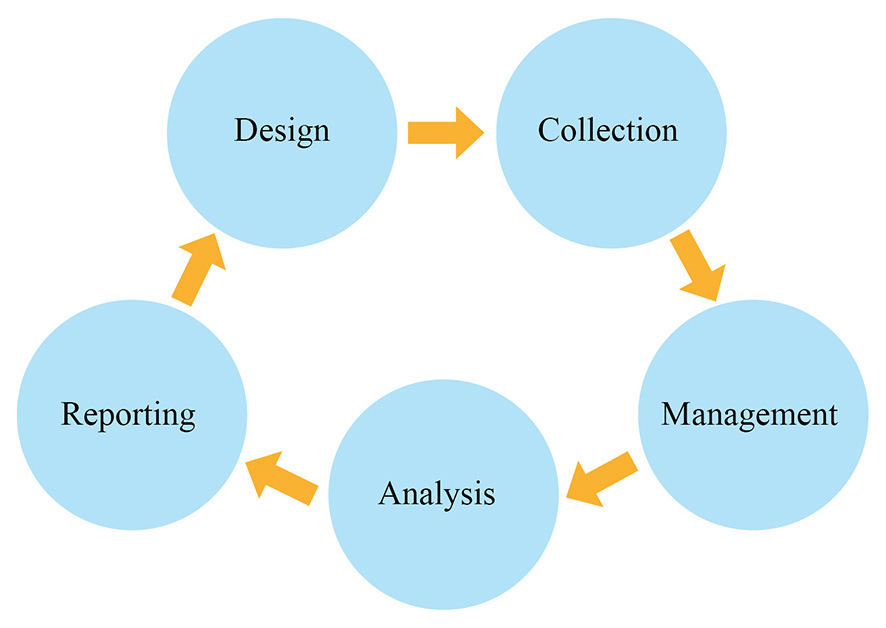
\includegraphics[width=0.75\textwidth]{literature/img/5stage.jpg}
	\caption{The 5 stages of survey research}
	\label{fig:literature:5stages}
	\end{figure}

	The authoring languages studied are focused on one or more stages of the survey research cycle. For instance, \gls{triples} and \gls{ddi} pay special attention to analysis and reporting stages since they provide structures that permit exporting the data collected for a questionnaire as well as its associated meta data. 
	In contrast, \gls{qdl} is best suited to address the design stage since it is built as part of a project to develop a tool for documenting questionnaire specifications \cite{man:bethlehem02}. 

	Whilst \gls{sss}, although was built to facilitate the creation of intuitive interfaces for supporting the design stage, it is more adequate to drive the collection stage given its formalism to describe expressions which offers more advantages than its counterparts and permits reducing the number of validations that have to be carried out before executing a questionnaire.
		
\section{CAWI Systems}\label{sec:literature:cawiSystems}
		\gls{cawi} systems are based on a \gls{cs} architecture style that uses \gls{http} to communicate between client and server. Several refinements for this basic architecture have been made over the years such as the \emph{distributed objects} style (e.g. \gls{corba}), which uses the object-oriented paradigm, for client server communication by encapsulating data and behaviour together \cite{proc:overdick07}. This approach is not appropriate for distributed environments since it asserts too much responsibility on the client which has to manage the life-cycle of objects, i.e. operations such as create, copy, move or destroy, and the server that has to rely on these operations performed.

	A more modern architecture style is \gls{soa} that defines services to address the different functionalities of a system. In this approach, there are two agents involved: the \emph{provider}, which implements a defined business function that operates independently of any other service provider; and the \emph{consumer} which uses the service \cite{tech:mackenzie06}. The interactions among the agents are performed through different communication protocols such as \gls{soap} and using standard exchangeable formats like \gls{xml}.

	As Pexel company demands the design and development of a new \gls{cawi} solution that can offer potential advantages over competitors, we consider that it is important to evaluate different architectural properties for the existing \gls{cawi} systems in order to determine how they address the simplicity, portability, reliability and scalability. Similarly, as the software system is network-based, it is crucial to review different test strategies for performance since these may help to estimate response times that in term, impact usability.

	The rest of this section is structured as follow: Section \ref{sec:literature:architectures} reviews the architectural style of different \gls{cawi} systems and Section \ref{sec:literature:performanceTesting} explores different testing methods and parameters used to simulate scenarios for performance testing of \gls{cawi} systems.





	\subsection{CAWI System Architectures}\label{sec:literature:architectures}
			This Section explores Blaise and SurveyMonkey architectures in order to determine the architectural properties being adopted by \gls{cawi} systems. However, other software solutions such as \gls{cases}, have not been explored due to the absence of publicly available documentation.

	\subsubsection{Blaise}\label{sec:literature:blaise}
	%This style permits developers to focus on a specific role, i.e. they can implement and maintain isolated services, multiple applications can reuse services code and the testability is improved.
	The architecture style of Blaise is \gls{wcf}, which is an implementation of \gls{soa}. In this style, the interactions among components is carried out by sending data through asynchronous messages that can be either \gls{xml} formatted or using complex streams of binary data. The \gls{cawi} solution offered by Blaise, separates the functionalities into different roles (see Figure \ref{fig:literature:soaBlaise}) \cite{proc:segel15}. The most important server roles are: \emph{survey manager}, that holds the creation and publishing of surveys; \emph{data entry server}, used to validate input and routing logic; \emph{data server}, that performs read/write operations into the databases; \emph{session server}, that stores and controls the active interviews; and \emph{web server} used to host and serve web pages to the end users. %This role uses the \gls{mvc} design pattern that offers benefits such as loose coupling due to the separation of concerns, it helps to manage the application when becomes more complex or promotes parallel development (e.g. one developer can focus on the model, a second can concentrate on the controller and a third one on the view). Nevertheless, we consider that this component can be moved to the client-side since browsers nowadays have mature JavaScript frameworks able to apply this design pattern. Hence, this suggestion may produce a much better user experience and help to reduce network latency since only data in \gls{json} or \gls{xml} format is sent.

	\begin{figure}[h]
	\centering
	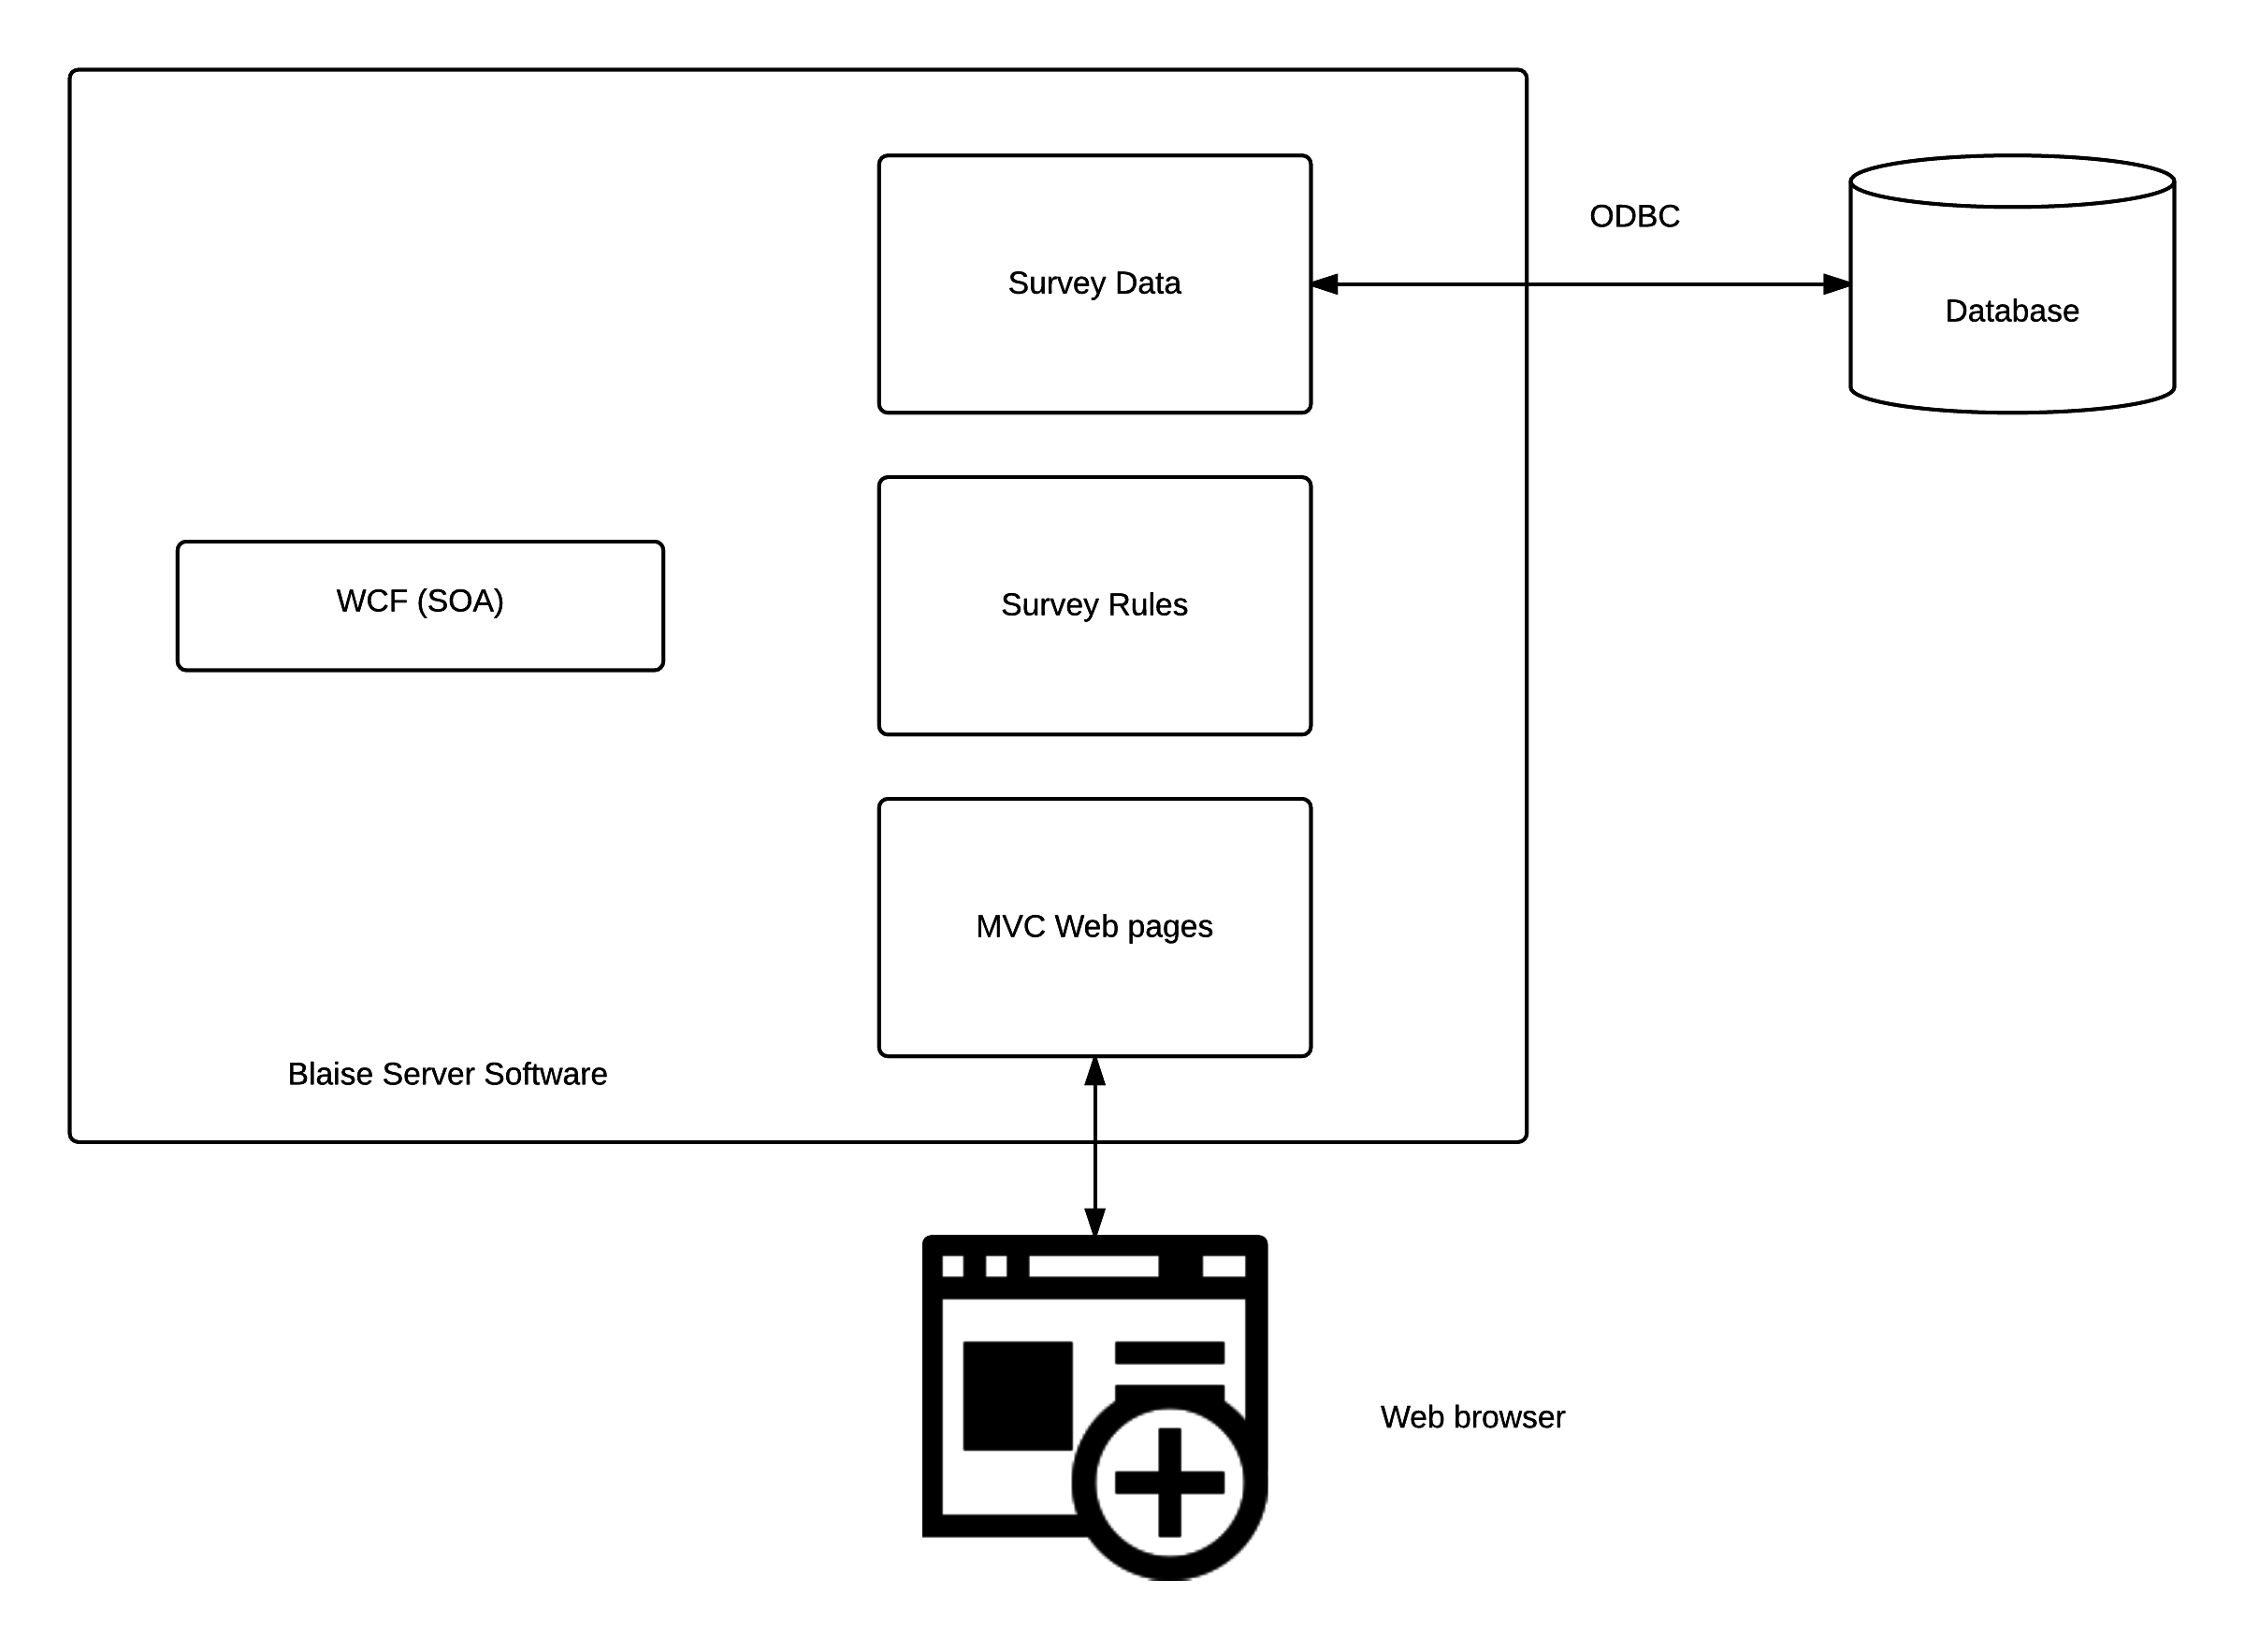
\includegraphics[max size={\textwidth}{\textheight}]{literature/img/soaBlaise.png}
	\caption{Blaise Architecture}
	\label{fig:literature:soaBlaise}
	\end{figure}

	The \gls{wcf} architecture style of Blaise induces simplicity by making a clear separation of concerns that leads to have services less complex and interdependent. Additionally, as this approach defines interfaces to communicate the different roles, any change at any component should not impact negatively into its consumers. However, the portability, reliability and scalability are not carefully considered. Specifically, the portability is not present due to the platform-dependent architecture of \gls{wcf} that only works under Microsoft environments. Regarding the reliability, it may be affected by the fact that the data server role makes the entire system vulnerable under any failure due to its inability to be set up with multiple physical or virtual machines \cite{proc:volguine13}. In respect to the scalability, the presence of a session server role to keep the state of every interview ongoing, not only prevents the server to free resources but also makes it harder to manage, replicate and synchronise state changes under a multi-server configuration.

	\subsubsection{SurveyMonkey}\label{sec:literature:surveyMonkey}
	%http://www.slideshare.net/mingli.yuan/a-brief-introduce-to-wsgi
	%http://agiliq.com/blog/2013/07/basics-wsgi/
	%https://developer.surveymonkey.com/api/v3/#authentication
	SurveyMonkey is the world's largest survey company \cite{web:groom14}. Its \gls{cawi} solution is written in Python and its core features are separated into different services. Most of the services communicate through a \gls{json} web \gls{api} over \gls{http}/\gls{http}S. SurveyMonkey implements \gls{soa} through \gls{wsgi} (see Figure \ref{fig:literature:surveyMonkey}). In this style, the web server is set up to receive client's requests and return responses back. The web server itself, does not directly creates a response but invokes the web application that produces a response based on the \gls{url} requested and pass it back to the web server. The server ultimately sends to the client. The \gls{wsgi} specifies the rules that need to be implemented by both sides, i.e. the web server and \gls{mvc} Framework. SurveyMonkey utilises Pyramid as the web application framework to produce many of its services.

	\begin{figure}[h]
	\centering
	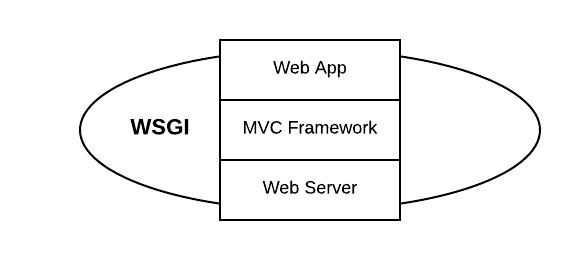
\includegraphics[width=0.75\textwidth]{literature/img/surveyMonkey.png}
	\caption{SurveyMonkey Architecture}
	\label{fig:literature:surveyMonkey}
	\end{figure}

	The \gls{wsgi} architecture style of SurveyMonkey induces simplicity and scalability. The simplicity is achieved through the use of pyramid \gls{mvc} web framework which permits loose coupling due to the separation of concerns. This software pattern, promotes parallel development (e.g. developers may focus on models, controllers or views). Regarding the scalability, unlike Blaise, there is no session persisted on the server, i.e. its stateless configuration based on a token-based authentication, promotes flexibility to scale. In respect to the portability, the application code is written in a cross-platform language, however we have not found enough information to determine whether or not the reliability or portability are induced. %For instance, the lack of awareness regarding its database solution



	\subsection{Performance Testing}\label{sec:literature:performanceTesting}
			\gls{cawi} systems are addressed for large group of respondents that can access simultaneously to complete a questionnaire at any time. As these systems are network-based applications, it is desired to conduct performance testing in order to determine the capacity of the system to work under different configurations.

	The performance testing consist of creating different test plans by varying parameters such as number of concurrent users or the complexity of the survey selected. Typically, the methodology plan to execute performance testing consist of:

	\begin{itemize}
		\item Selecting a survey, where the length and complexity helps to predict the performance of the system to deal with questionnaires with similar constructs.
		\item Designing a specific scenario either by randomly responding to questions or by taking the most common sequence of questions answered by survey respondents \cite{proc:volguine13}.
		\item Varying the number of concurrent respondents and finally running the scenario under the parameters chosen.
	\end{itemize}

	Segel et al. discuss a \emph{stress test} strategy in order to verify the capacity of a web deployment of Blaise system \cite{proc:segel13}. In that experiment, they vary the number of concurrent respondents and introduce the \emph{thinking time} concept consisting of setting up a random distributed time that simulates the amount of time that takes respondents to answer questions. Additionally, they explain the importance of selecting an adequate time in which the maximum number of concurrent users will be reached in order to avoid unrealistic simultaneous accesses.

	A more recent study carried out by Volguine pursues a stable and responsive on-line survey respondent experience through the introduction of three more test strategies a part from stress testing. These are: \emph{normal capacity} consisting in monitoring the system for two hours under an average load level for a day, \emph{peak} during two hours under a maximum load expected for day and \emph{endurance} with a significant load level during eight hours \cite{proc:volguine13}. Although Volguine offers a full suite of tests to assess performance, reliability and responsiveness of Blaise, it is not clear whether the thinking time is included or not. Therefore, this can lead to a biased testing situation that is not close to a real scenario in which an interviewee thinks before responding to a question. Moreover, the use of normal, peak and endurance tests strategies assumes that the tester knows what are the system level usages which is not always known, specially for \gls{cawi} systems that have never been in the market.

\section{Conclusions}
		Our \gls{cawi} system solution for survey life-cycle adopts \gls{rest} constraints to adhere to scalability, simplicity and reliability architectural properties expected for \gls{cawi} systems. Particularly, the \gls{rest} \gls{api}, which conforms to the \gls{http} protocol, has been implemented with the standard reference library for Java. This multi-layered solution is highly portable and uses a \gls{nosql} database solution which permits a more flexible persistence solution when compared to the traditional relational databases.

	The client side, based on the \gls{spa} not only improves the responsiveness of a distributed system but also helps to produce richer interactive interfaces. This paradigm when compared to the multi-page approach that \gls{cawi} systems such as Blaise or SurveyMokey adopt, is more attractive. Particularly, with the choice of AngularJS as the framework for building pages, we have gained a simplified cross browser testing of functionalities, reduced the server burden by transferring interface logics to the client and promoted a parallel development of design and collection interfaces.





